%preamble
\documentclass[letterpaper]{article}
\synctex=1
\usepackage{graphicx}
\graphicspath{ {images/} }

\usepackage{lipsum}
\usepackage{float}
% \bibliographystyle{IEEEtran}
\bibliographystyle{ieeetr}

\usepackage{amssymb}

\usepackage{siunitx}
%actual document
\begin{document}

  % \maketitle %insert titlepage here
  \begin{titlepage}
    \begin{center}
        \vspace*{1cm}
        \Huge
        Experiment 4
        \vspace{1cm}

        Magnetic Fields
        \vspace{1cm}

        By: Arun Woosaree
        \vspace{1cm}

        Lab partners:
        \vspace{.25cm}
        \Large

        Fatemeh Ghafari Far\\
        % Purvish Jajal
        \vspace{.25cm}
        Yvonne Hong
        \vspace{1cm}

        \Huge
        PHYS 230 Lab EH71
        \vspace{1cm}

        TA: Andrei Tretiakov
        \vspace{1cm}

        Date of Lab: March 22, 2018%\today
        \vfill
    \end{center}
\end{titlepage}

\section{Introduction}
% Begin with experiment’s objectives\\
% Give physical background:\\
% ○ Describe investigated/used\\
% phenomena e.g. Gauss’s law,\\
% field lines, equipotential lines.\\
% ○ Do not copy text from a
% textbook/manual\\
% Provide equations you used\\
% ○ Identify all symbols\\

In this experiment, we measure the distribution of the magnetic field across a solenoid, and
we also measure the magnetic field of a Helmholtz coil, from which we experimentally determine the
number of turns of the wire in the coil. The right hand rule is used to determine the
direction of the magnetic $\textbf{B}$ field in the coils of wire. The right handed rule
is defined as follows: the four main fingers of one's right hand curls in the direction of the
current in the wire, and the resulting direction in which the thumb points is the direction of the
$\textbf{B}$ field.
\textbf{By doing shit, and using these equations, we can determine other shit, and then
we can see even more shit by plotting a graph using a linearized version of this
shit equation}
The electrons are emmitted from a hot filament, accelerated by an electric field, and then deflected
by a magnetic field into a circular orbit. If the radius of this orbit is known,
as well as the intensity of the magnetic field, and the accelerating potential of the
electric field, we can determine $e/m$ and the velocity $v$ of the electrons, and an approximate value for
the earth's magnetic field $B_E$. Using the left-hand-rule for moving charge (since we are
dealing with electrons), we can also figure out the direction of the magnetic field which deflects the electrons.
The charge to mass ratio is found using the following equation, of which a derivation exists in the Discussion section.
The equation below is also linearized, and graphed, from which we obtain an approximate value of the earth's magnetic field using the
Y-intercept, and $e/m$ from the slope.
\begin{equation}
  B=\frac{1}{2}\mu_0nI(\cos{\Beta_2}-cos{\Beta_1})
\end{equation}
In this equation, $e$ is the charge of an electron, and $m$ is the mass of the electron, `V' is the DC voltage applied to the Helmholtz coil
, $B_H$ is the magnetic field of the coil, given by
\begin{equation}
  B_c=\frac{\frac{1}{2}\mu_0NR^2I}{(R^2+(x-x_c)^2)^{\frac{3}{2}}}
\end{equation}
\begin{equation}
  B_H=\frac{8\mu_0NI}{\sqrt{125}R}
\end{equation}
,and r is the orbit radius of the electrons. In Equation 2 above, $\mu_0$ is the permeability permeability of free space,
$N$ is the number of turns in the Helmholtz coil, $R$ is the radius of the coil, and $I$ is the measured current through the
coil.

\section{Experimental Method}
% List all equipment used\\
% ○ Provide parameters as detailed as
% possible: masses, frequencies,
% etc.\\
% Report what YOU DID to achieve
% experimental goals:\\
% ○ Do not use imperative clause\\
% ○ Use first person narrative or
% passive voice\\
% Based on this section you should be
% able to reproduce your results without a
% manual

%use p1-2 and p2-3 to show setup
\textbf{List of Equipment:}
\begin{itemize}
  \item Helmholtz coil apparatus (Figures 1 and 2)
  \item AC Voltage Source
  \item DC Voltage Source
  \item Voltmeter
  \item Ammeter
  \item Wires
\end{itemize}

\begin{figure}[h!]
    \centering
    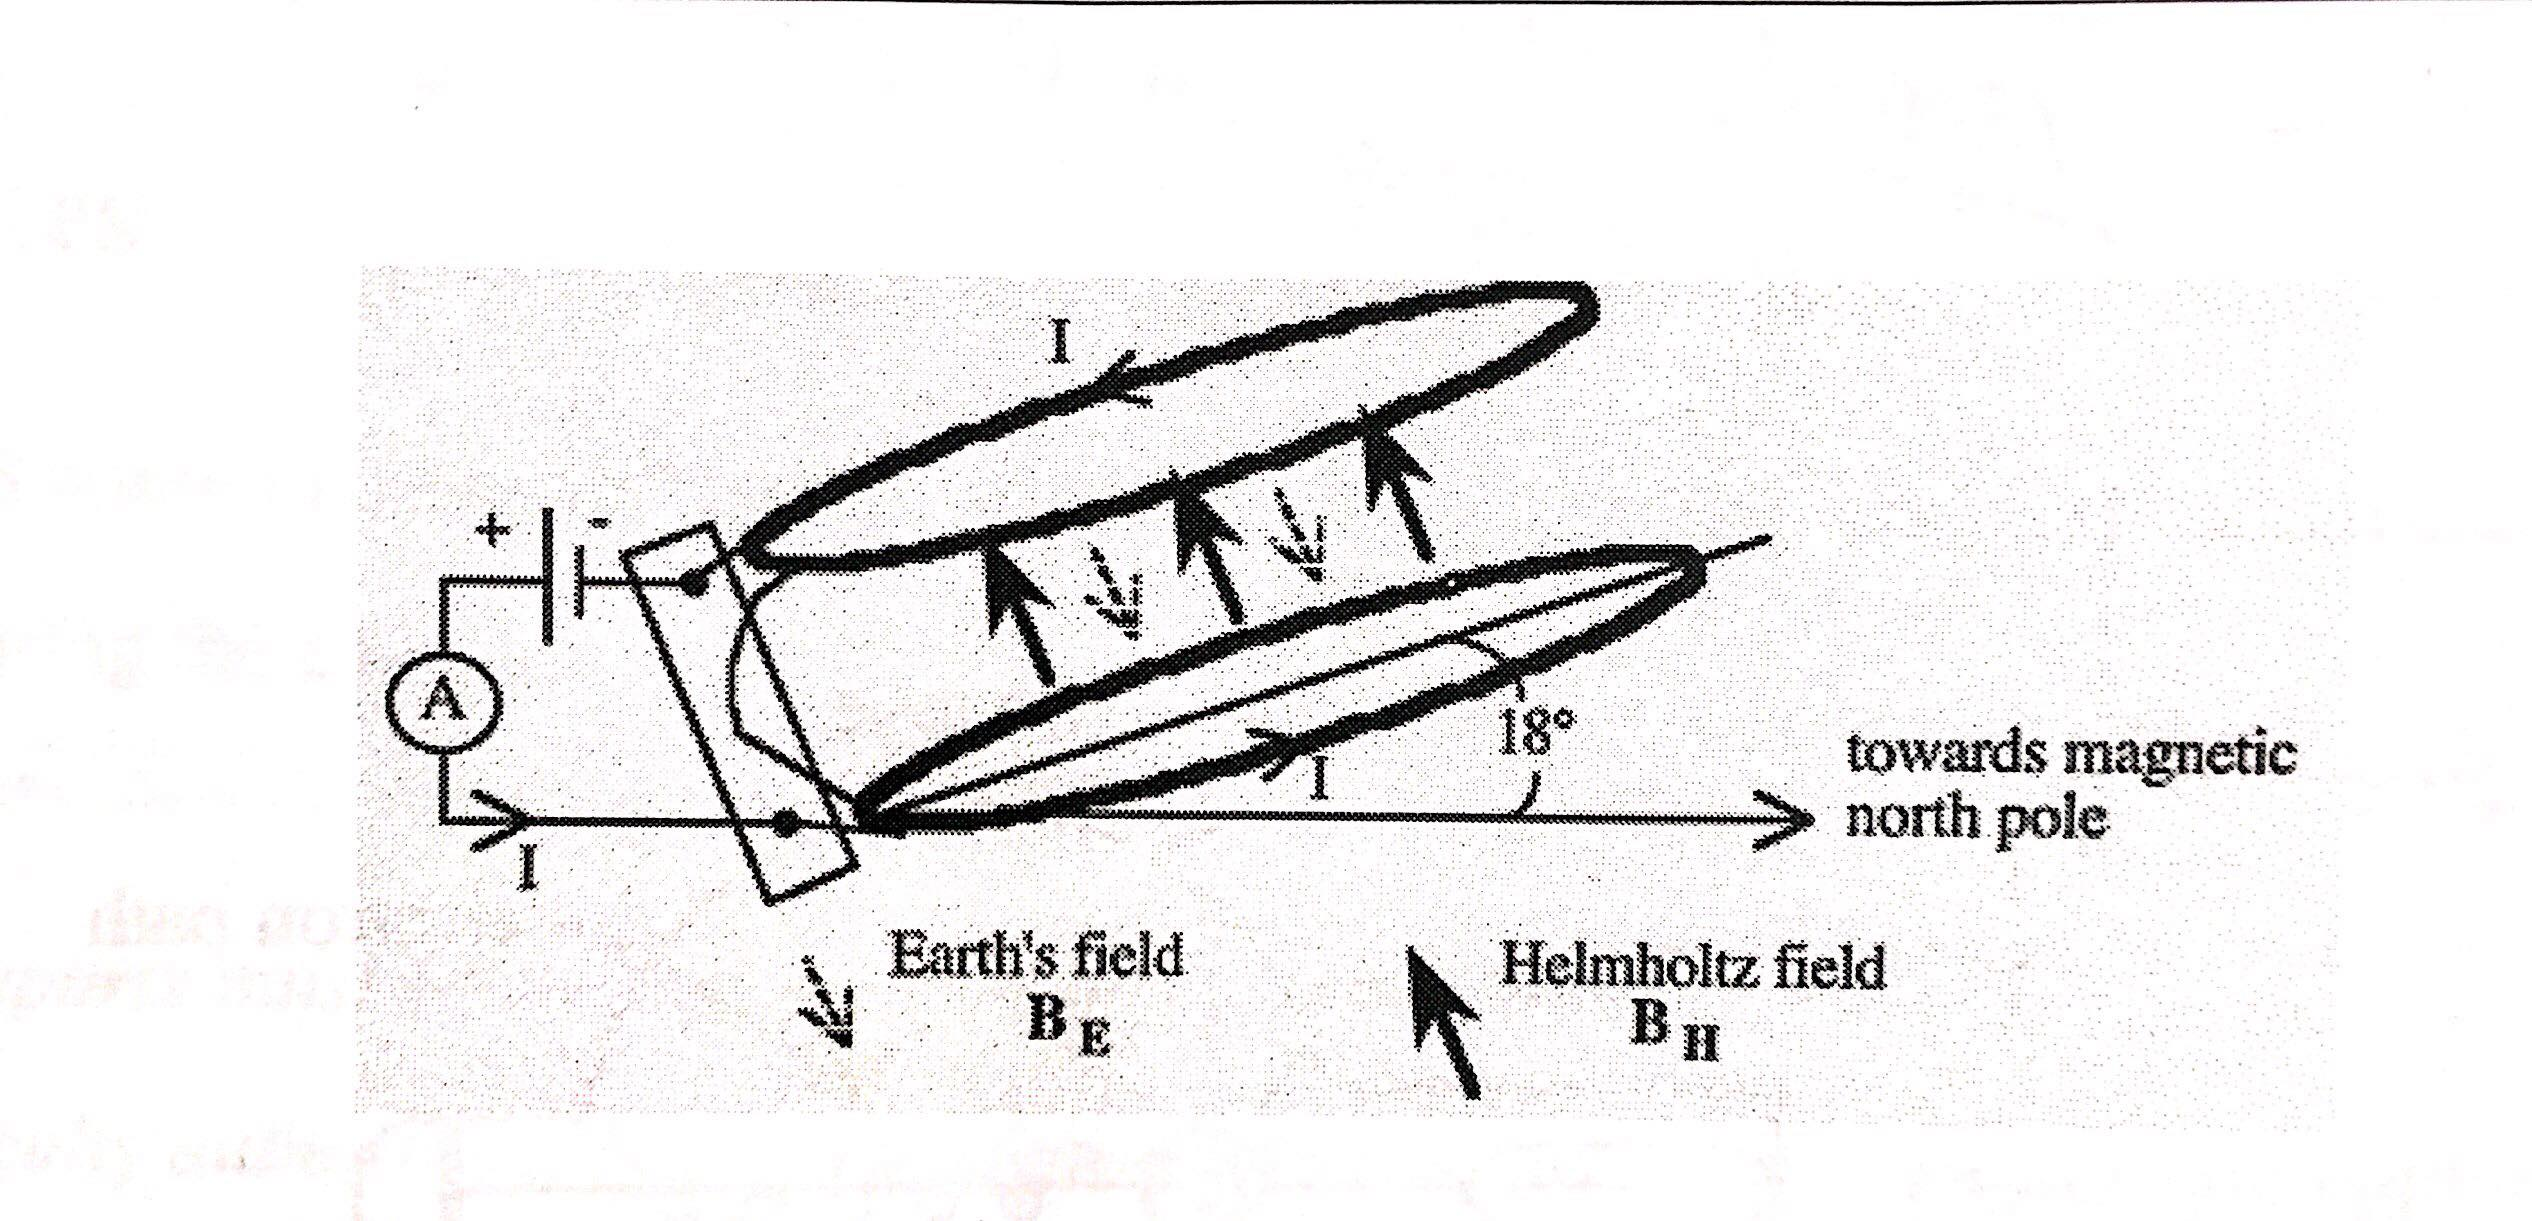
\includegraphics[width=\textwidth]{fig1.jpg}
    \caption{Helmholtz coil apparatus, and its alignment opposite to earth's magnetic field. \cite{labmanual}}
\end{figure}

The Helmholtz coil was set up such that its alignment is approximately
opposite to the Earth's magnetic field, which in Edmonton means that the coil
should be tilted upwards at an angle of about 18 degrees relative to the horizontal.
\begin{figure}[h!]
    \centering
    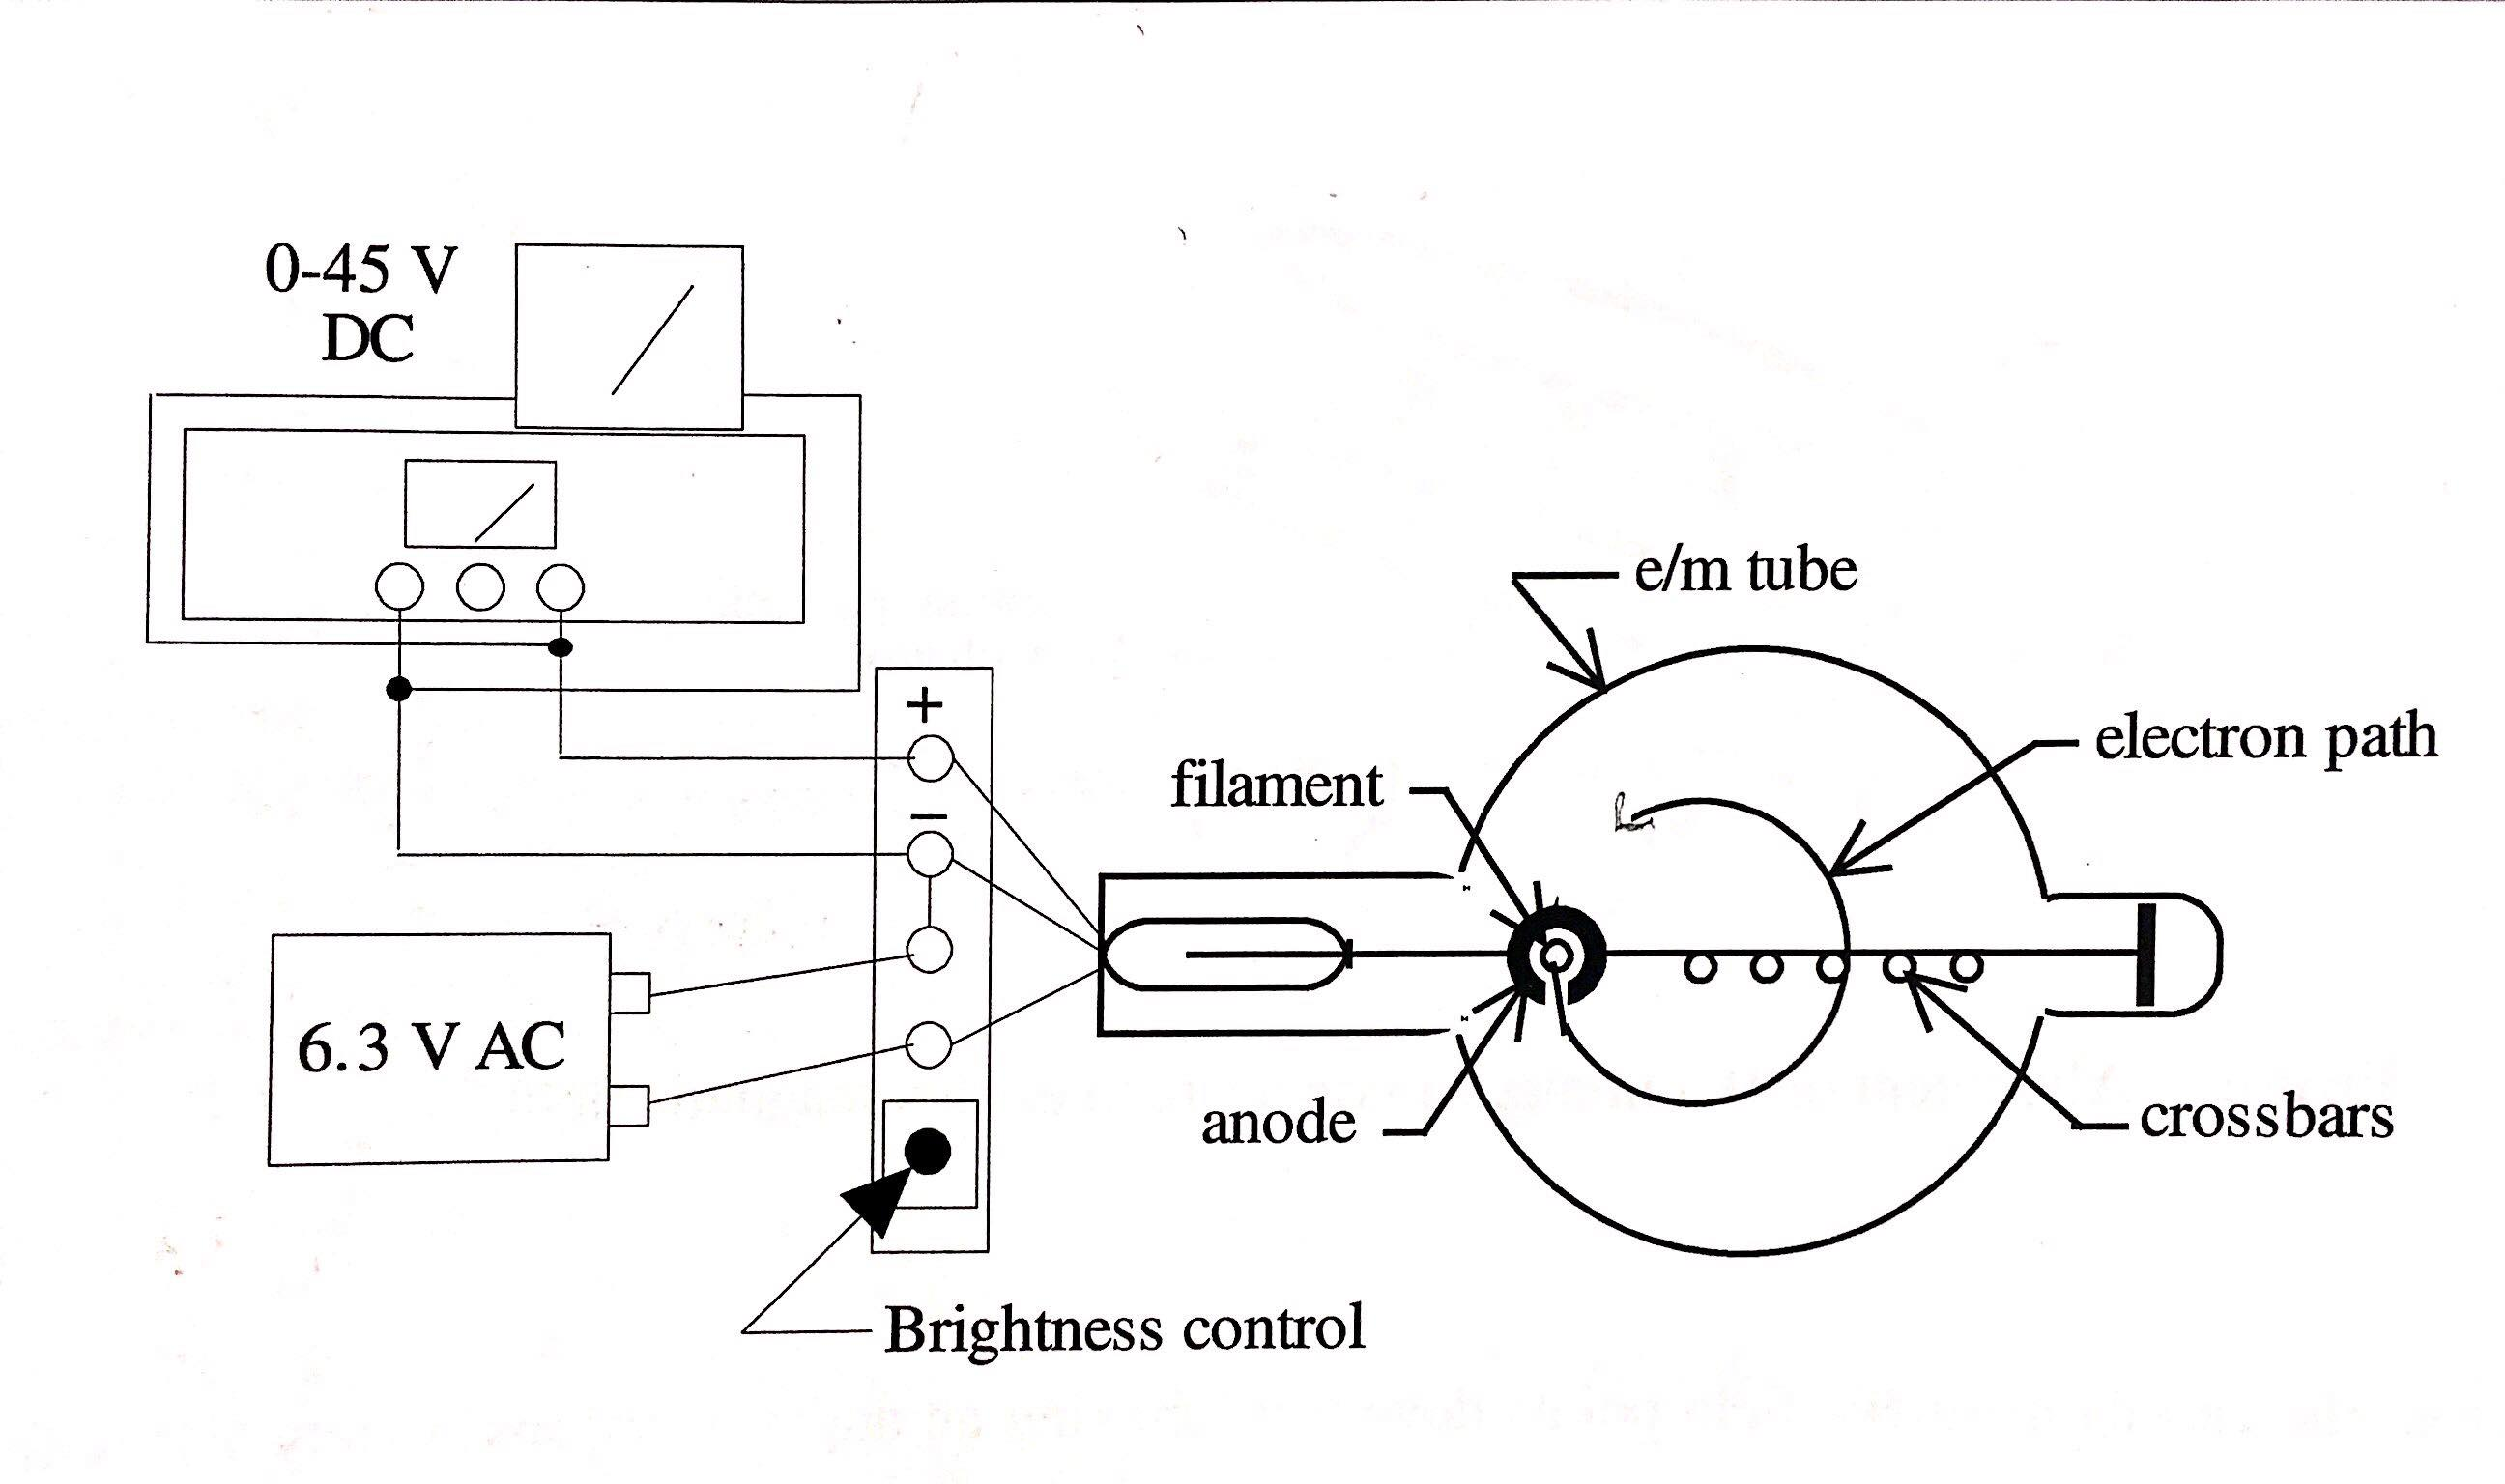
\includegraphics[width=.9\textwidth]{fig2.jpg}
    \caption{Circuit wiring for the apparatus \cite{labmanual}}
\end{figure}
The apparatus involves three separate electrical circuits.
The filament, anode circuit, and the Helmholtz circuit are connected as outlined
below in Figure 2. We first begin by setting the DC voltage source to 20 V, then modifying the
AC voltage source to change the radius of the glowing circular electron path. The current going through the
Helmholtz coil is recorded in a spreadsheet at each point where the loop is on the far side of each peg, with larger
currents resulting in smaller loops. Then,
the DC voltage source is set to 30 V, and the Helmholtz current $I$ is measured and recorded at the 5 points again.
The same process is repeated once more when the DC voltage source is set to 40 V. It should be noted
that adjusting the brightness control knob, viewing the loop from above, and doing the experiment in a dark
environment made it easier to view the electron loop.
Since we have the Helmholtz currents, and the diameter of the pegs in the apparatus are known (and therefore
the radius of the loops that the electrons make), a linear graph can be created by linearizing equation 1,
from which we can obtain the charge to mass ratio $e/m$ from the slope, and the earth's magnetic field $B_E$
from the Y-intercept.

\section{Results}

Raw data recorded while measuring the Helmholtz current \textit{I} required
to align the beam with the far side of each peg.

\begin{table}[H]
\centering
\begin{tabular}{|l|l|l|l|}
\hline
Voltage (V) & Current (A) & Peg number & Radius r (cm) \\ \hline
20          & 2.68        & 1          & 0.0325        \\ \hline
20          & 2.19        & 2          & 0.039         \\ \hline
20          & 1.94        & 3          & 0.045         \\ \hline
20          & 1.73        & 4          & 0.0515        \\ \hline
20          & 1.54        & 5          & 0.0575        \\ \hline
30          & 3.12        & 1          & 0.0325        \\ \hline
30          & 2.66        & 2          & 0.039         \\ \hline
30          & 2.29        & 3          & 0.045         \\ \hline
30          & 2.1         & 4          & 0.0515        \\ \hline
30          & 1.9         & 5          & 0.0575        \\ \hline
40          & 3.62        & 1          & 0.0325        \\ \hline
40          & 3.05        & 2          & 0.039         \\ \hline
40          & 2.63        & 3          & 0.045         \\ \hline
40          & 2.35        & 4          & 0.0515        \\ \hline
40          & 2.12        & 5          & 0.0575        \\ \hline
\end{tabular}
\caption{Raw data recorded when measuring the Helmholtz current}
\end{table}


Using the data in Table 1, a linear graph is generated with Equation 1,
which is obtained through a derivation outlined in the discussion section.
\\The equation is linearized by the following process:
$$ B_H = \frac{8\mu_0NI}{\sqrt{125}R} $$
$$ \Therefore B_H= \frac{8 (\SI{4\pi e-7}{\tesla\metre\per\ampere})}{\sqrt{125}(\SI{14.8}{\cm})} $$
$$ \Rightarrow N = \frac{B_H \sqrt{125} R}{8\mu_0I} $$
$$ \therefore N= \frac{} $$
 so we generate a graph
with $\frac{\sqrt{2V}}{r}$ on the X axis using our measured voltage values, and $B_H$ on the Y axis
using our measured current values.

\begin{figure}[H]
  \centering
  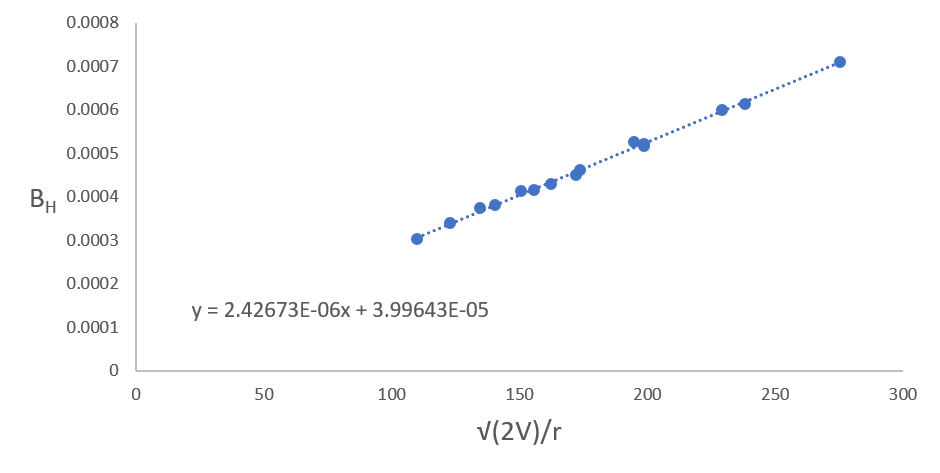
\includegraphics[width=\textwidth]{chart1.png}
  \caption{Measuring the voltage difference in a region between two parallel conductors.}
\end{figure}

\newpage
\noindent Using Excel's LINEST function, we obtain the following data from the graph in Figure 3.
\begin{table}[H]
\centering
\begin{tabular}{cc}
  Slope $\sqrt{m/e}$ : &  $\num{2.4267255938411E-06}\pm \num{3.50649774570897E-08}$ \\
  Y-Intercept $B_E$   :&  $\num{3.99642631798173E-05}\pm \num{6.40167504007098E-06}$ \\
\end{tabular}
\caption{LINEST data from the graph in Figure 3}
\end{table}

\noindent To obtain the calculated value for $e/m$, we can see from our LINEST data (Table 2) that the slope, $\sqrt{m/e}$ is
$\num{2.4267255938411E-06}$.\\
Thus, the calculated value of $e/m$ can be found:
$$ \frac{e}{m} = \left(\sqrt{\frac{m}{e}}\right)^{-2} = 1.69808200223924714236 \times 10^{11} $$
And the error $\delta \frac{e}{m}$ can be calculated using partial derivatives:
$$slope= \left(\frac{e}{m}\right)^{-1/2}$$
$$\delta slope = \left| -\frac{1}{2} \left(\frac{e}{m}\right)^{-3/2} \delta \left(\frac{e}{m}\right)\right|$$
$$ 2 \times \delta slope = \left(\frac{e}{m}\right)^{-3/2} \delta \left(\frac{e}{m}\right) $$
$$ \therefore \delta \left(\frac{e}{m}\right) = 2 \times \delta slope \left(\frac{e}{m}\right)^{3/2}$$
From our LINEST data (Table 2), we know that $\delta slope = \num{3.50649774570897E-08} $
$$ \therefore \delta \left(\frac{e}{m}\right) = 2 \times \num{3.50649774570897E-08} \times (\num{1.69808200223924714236e11})^{3/2}$$
$$= \num{4.90728801640585e9} \approx \num{4.91e9}$$
Thus, the calculated value for $\frac{e}{m}$ is:\footnote{Value rounded to three significant digits simply for neatness. Otherwise, the full values were messy and long}
$$\frac{e}{m}=\num{1.70e11} \pm \SI{4.91e9}{\coulomb\per\kilogram}$$
The percent error is:
$$ \frac{|\num{1.69808200223924714236e11}-\num{1.76e11}|}{\num{1.76e11}}\times100 = 3.52\%$$
Obtaining the calculated value and error for $B_E$ is a much simpler matter. We simply
look at the data generated by LINEST, specifically, the Y-intercept (Table 2).
$$B_E = \num{4.00E-05}\pm \SI{6.40E-06}{\tesla}$$
The percent error is:
$$ \frac{|\num{3.99642631798173E-05}-\num{4.8e-5}|}{\num{4.8e-5}}\times100 = 16.74\%$$

\vspace{1cm}
\noindent The calculated values of $e/m$ and $B_E$ from the graph are summarized in Table 3.
\begin{table}[H]
\centering
\begin{tabular}{c|c|c|c|}
                & Expected                      & Calculated:                                     & \% Error \\ \hline
$e/m$: & $\SI{1.76e11}{\coulomb\per\kilogram}$      & $\num{1.70e11} \pm \SI{4.91e9}{\coulomb\per\kilogram}$  &    $3.52$  \\ \hline
$B_E$: & $4.8 \pm \,\SI{0.3e-5}{\tesla}$           & $\num{4.00e-5} \pm \,\SI{6.40e-6}{\tesla}$                    &   $16.74$  \\ \hline
\end{tabular}
\caption{Measured values of $e/m$ and $B_E$ compared to the calculated values obtained from the graph.}
\end{table}

\section{Discussion}

\subsection{Part 1}


From Table 3, we can see that our calculated values for $e/m$
($\num{1.70e11} \pm \SI{4.91e9}{\coulomb\per\kilogram}$)
and $B_E$
($\num{4.00e-5} \pm \,\SI{6.40e-6}{\tesla}$) were in the same order of magnitude as the
expected values. ( $\SI{1.76e11}{\coulomb\per\kilogram}$ for $e/m$
and $4.8 \pm \,\SI{0.3e-5}{\tesla}$ for $B_E$.)
Additionally, the percent error for the charge to mass ration seemed relatively good, being 3.52\%.
However, our calculated value of $B_E$ was a fair bit off, with a 16.74\% error.
Unfortunately, it is clear that our calculated values do are not within error of the
expected values.

At first glance, the graph (Figure 3) produced from our raw data (Table 1) seems reasonable, especially
because all the data points recorded seem to fit nicely on the trendline with
no anomalous data points compared to the other values. This means that whatever error
introduced in our measurement of voltages was a constant factor, since we took care
to measure the currents exactly when the electron loop was on the far side of each peg, as specified in the
lab manual. There are many potential sources of error, including human error, and potential miscalibration of equipment since we are dealing
with electrons which are tiny in nature. We did our best to keep these factors constant.

\begin{figure}[H]
  \centering
  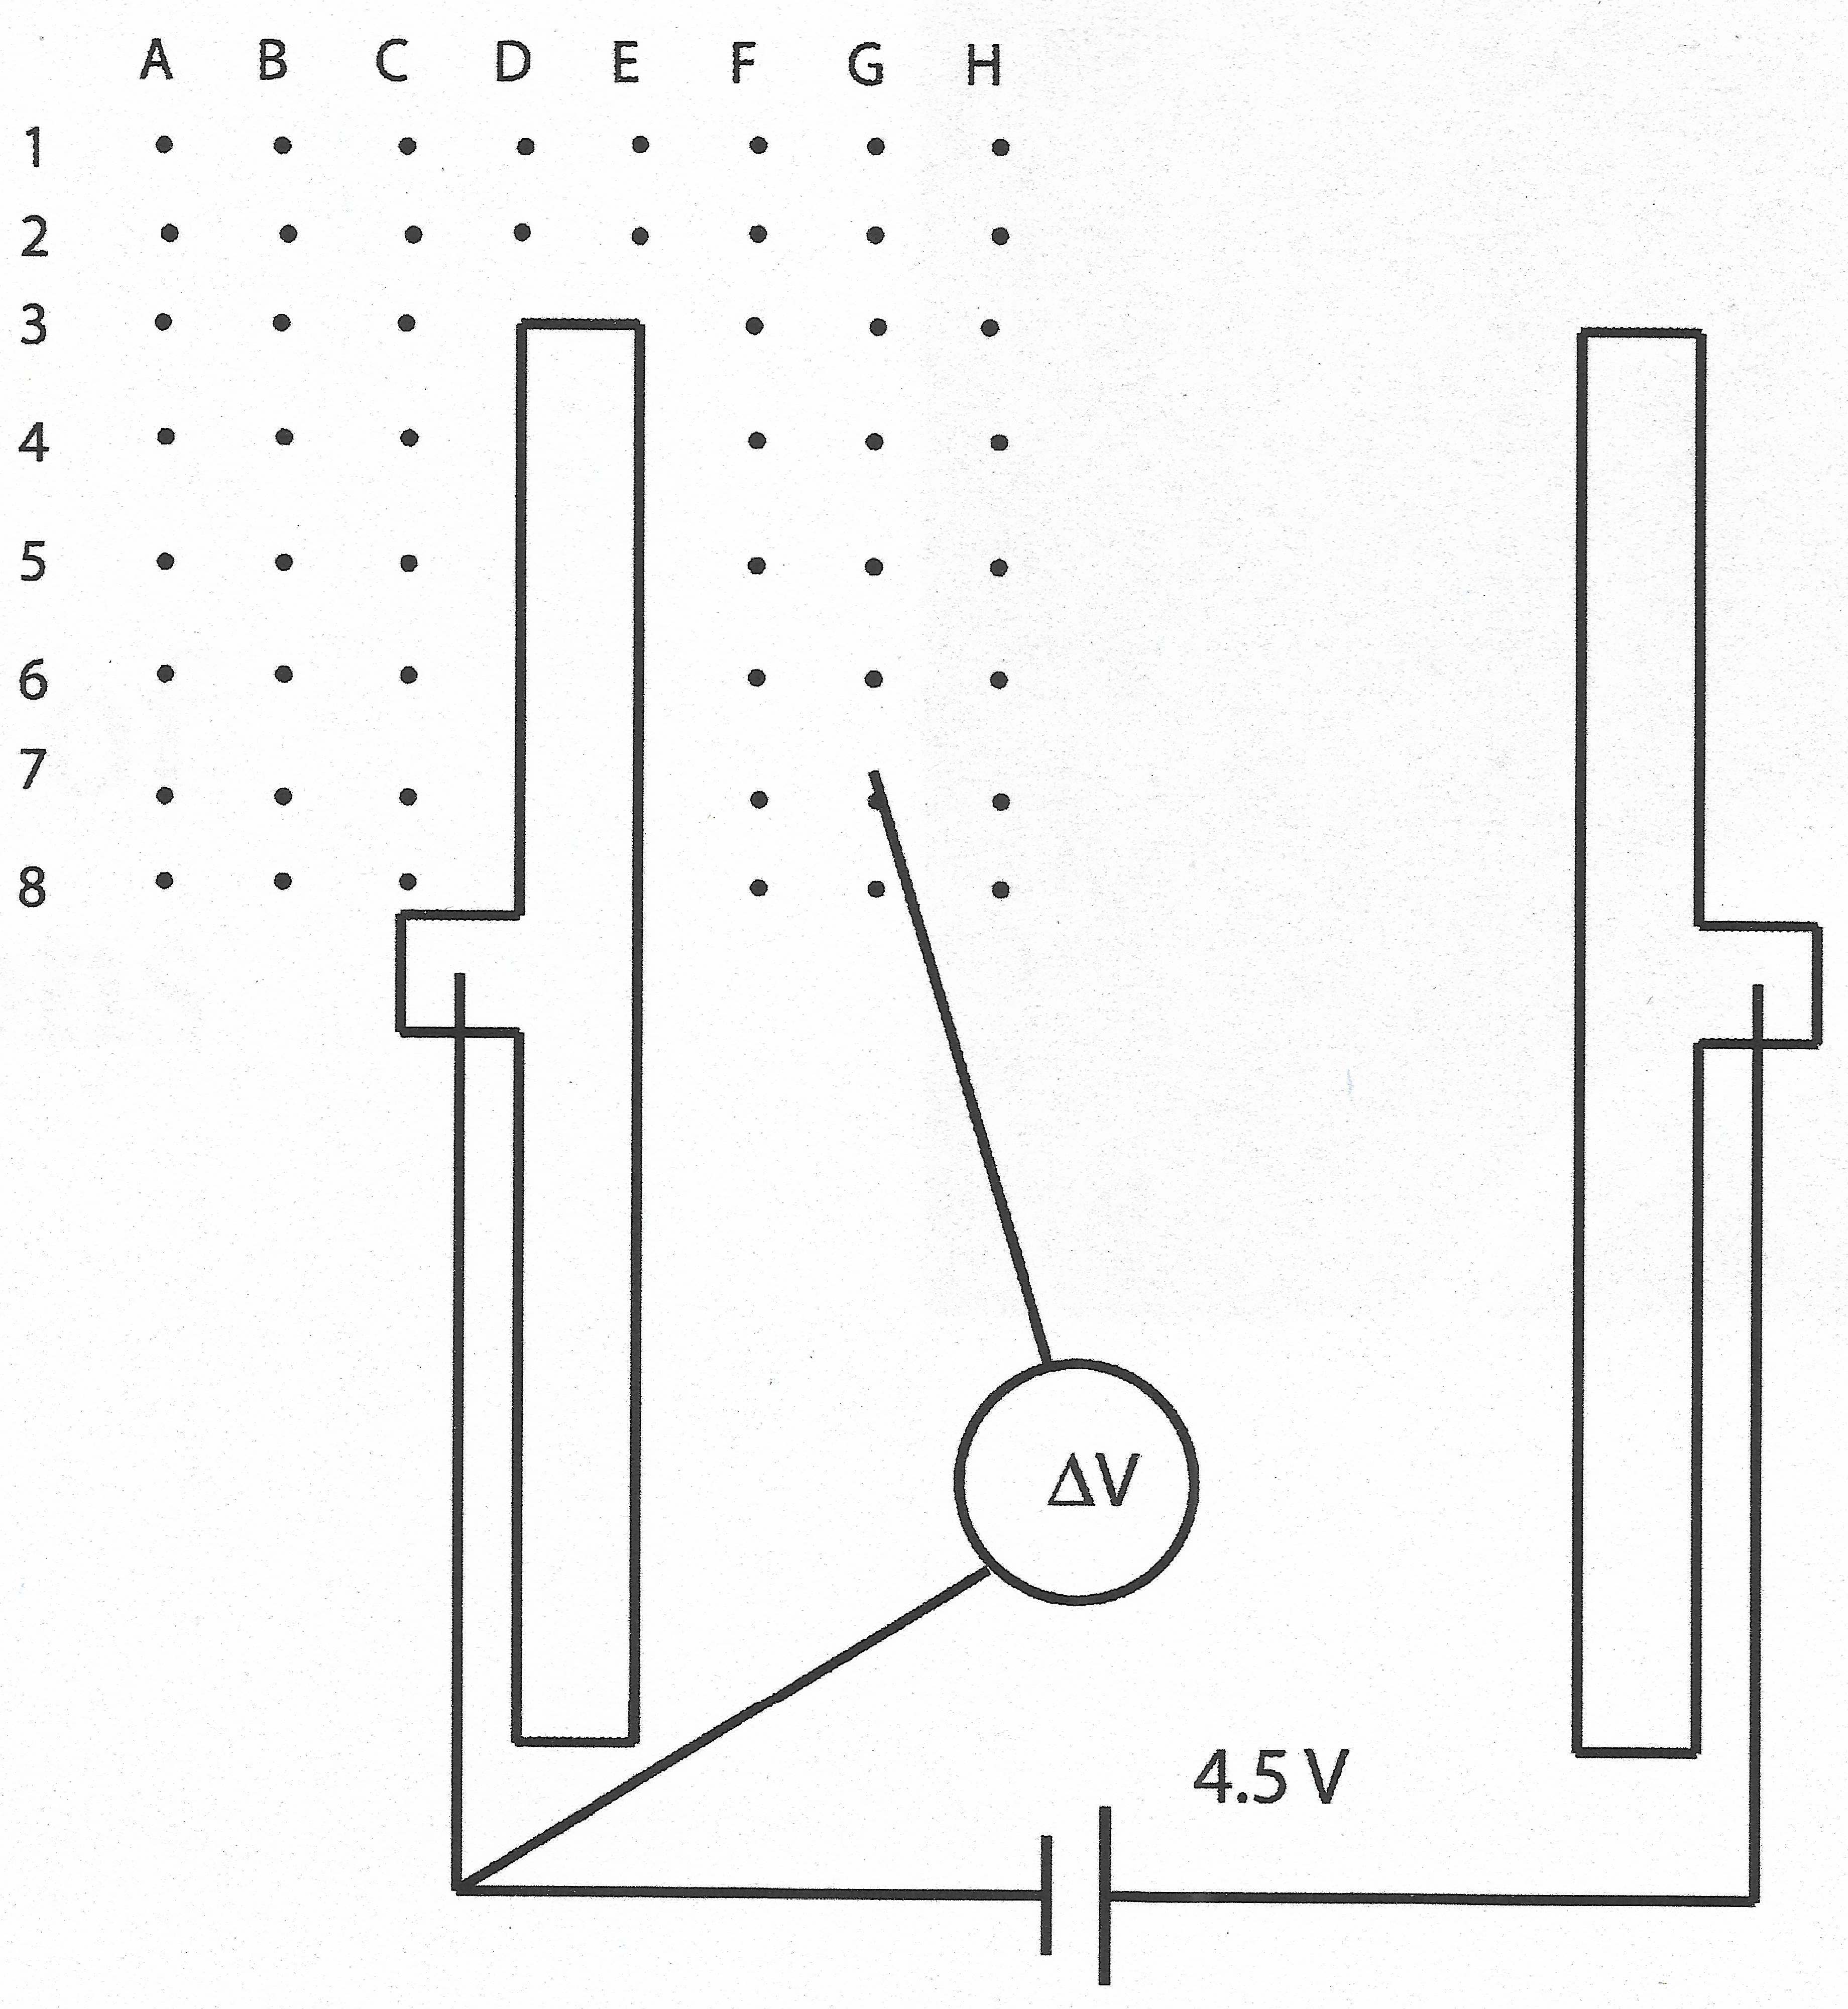
\includegraphics[width=\textwidth]{fig3.jpg}
  \caption{The direction of the \textbf{B} field is found to be pointing out of the page when drawn this way.}
\end{figure}

Using the left-hand-rule for moving a charged particle, (since we are
dealing with electrons which have a negative charge), we determine that the net magnetic field \textbf{B}
points upward, perpendicular to the radius of the coil, or upwards relative to Figure 2. Additionally, we notice that
as the Helmholtz current is increased a tighter loop is formed.

Equation 1, which which was manipulated to produce our graph can be derived using the following equations:

\noindent When a stream of electrons are accelerated through a potential difference $V$, the maximum
kinetic energy is given by:
$$\frac{1}{2}mv^2 = eV$$
Next, the Lorentz force \textbf{F} is given by:
$\textbf{F}=q\textbf{v}\times \textbf{B}$
(where $q$ is the charge of the moving particle), and since our magnetic field is set up so that \textbf{B} is perpendicular to the motion of the electrons (see Figure 1),
the magnitude of the force $F$ is given by $$F=qvB$$
Next, the radius of the circle, which is the path of the electrons in this experiment is such that
the centripetal acceleration is furnished by the Lorentz force. Therefore, we obtain $$\frac{mv^2}{r}=evB$$

\noindent To obtain Equation 1, we first rearrange the first of the three equations above and substitute it into the third.
$$\frac{1}{2}mv^2 = eV \Rightarrow v=\frac{\sqrt{2eV}}{m}$$
$$\Rightarrow \frac{m(\frac{2eV}{m})}{r}=e\sqrt{\frac{2eV}{m}}B$$
$$\Rightarrow \frac{4V^2}{r^2}=\frac{2eV}{m}B^2$$
$$\Rightarrow \frac{e}{m} = \frac{2V}{r^2B^2}$$
Finally, we notice that since our apparatus is aimed antiparallel to earth's magnetic field, such that
the magnitude of the total magnetic field $B=B_H-B_E$, and substitute this result in the above equation.
Finally, we obtain equation 1.
$$\frac{e}{m} = \frac{2V}{(B_H-B_E)^2r^2}$$

\textbf{Questions: }\\ \\
\textit{Why is it important to align the Helmholtz coil, so that its field is
        anti-parallel to the earth's magnetic field?}\\
\textbf{A:}
Earth's magnetic field is strong enough to deflect our little electron beam, which means its effects are non-negligible.
However, if we align our Helmholtz coil such that it is exactly anti-parallel to the Earth's magnetic field, we notice that
in this arrangement, since $B_E$ is pointing in the opposite direction to $B_H$, the magnitude of the net magnetic
field can be found simply by subtracting $B_E$ from $B_H$ since
it is anti-parallel to the earth's magnetic field. If the alignment was different, the geometry would not be so simple, and
the path of the electrons would not be in the same plane as the orientation of the Helmholtz coil.\\ \\
\textit{Explain what would happen if the beam in this experiment contained several ions of different masses.}\\
\textbf{A:}
If there were several ions of different masses, the ions with larger mass would
have a larger radius of curvature, and the ions with smaller mass would have a smaller radius of curvature, by observing that
the centripital force depends on the  $F_c=\frac{mv^2}{r}$ relation. By rearranging this, we see that
the mass is directly proportional to the radius of curvature, i.e. $m\propto r$.
Experimentally, we would notice that the glowing path of the ions would be wider, and therefore it would be difficult to measure
the Helmholtz currents exactly at the far side of the pegs in the apparatus, like we did for the electrons, which had unvarying masses.
This ambiguity would also skew our measured charge to mass ratio, since the charged masses are varied and not constant.

\section{Conclusions}
In Experiment 2, we calculate the charge to mass ratio $e/m$ of electrons fired in a Helmholtz coil, which are accelerated by an electric field, and
deflected by a magnetic field to form a circular orbit. The apparatus
was set up such that the magnetic field of the coil is aligned antiparallel to the earth's own magnetic field
to simplify the geomery. The current was varied at three diferent voltages to align the electron loops to known radii, so that we could use the
Helmholtz curents to calculate a value for $e/m$, and the earth's magnetic field $B_E$ by ploting a linear graph. We noticed that the
radius of curvature of the electron loops increased as the Helmholtz current was lowered. Additionally, using the
left hand rule (since electrons are negatively charged masses), we verified that the net magnetic field of the
setup was directed upwards, in the same orientation of the coil (in other words, the direction of the net magnetic field
was perpendicular to the radius of the coil). We calculated the charge to mass ratio of the electron to be ($\num{1.70e11} \pm \SI{4.91e9}{\coulomb\per\kilogram}$)
and the earth's magnetic field to be
($\num{4.00e-5} \pm \,\SI{6.40e-6}{\tesla}$). While these values are in the same order of magnitude as the
expected values ( $\SI{1.76e11}{\coulomb\per\kilogram}$ for $e/m$
and $4.8 \pm \,\SI{0.3e-5}{\tesla}$ for $B_E$), these values do not agree within error. The
graph generated from our data was linear, however, so it is likely that the source of error introduced was a
constant factor, whether it's miscalibration of equipment, or human error since we took care to record our
results in a consistent manner.

\bibliography{references}
\end{document}
